\documentclass[tikz,border=8pt]{standalone}
\usepackage[T1]{fontenc}\usepackage{lmodern,amsmath,amssymb}\usetikzlibrary{arrows.meta,positioning}
\begin{document}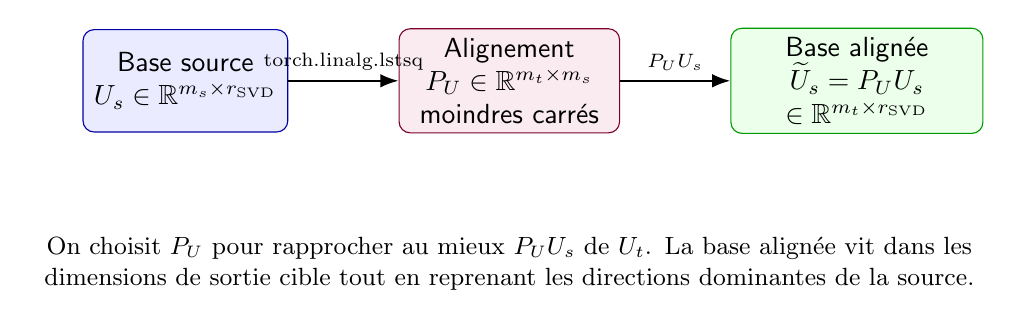
\begin{tikzpicture}[font=\sffamily,>=Latex,src/.style={draw=blue!65!black,fill=blue!8,rounded corners,minimum width=2.6cm,minimum height=1.3cm,align=center},map/.style={draw=purple!65!black,fill=purple!8,rounded corners,minimum width=2.8cm,minimum height=1.3cm,align=center},alignedbase/.style={draw=green!60!black,fill=green!8,rounded corners,minimum width=3.2cm,minimum height=1.3cm,align=center},arr/.style={-{Latex},thick}]
\node[src] (u) {Base source\\$U_s\in\mathbb R^{m_s\times r_{\rm SVD}}$};
\node[map,right=14mm of u] (p) {Alignement\\$P_U\in\mathbb R^{m_t\times m_s}$\\moindres carrés};
\node[alignedbase,right=14mm of p] (ut) {Base alignée\\$\widetilde U_s=P_UU_s$\\$\in\mathbb R^{m_t\times r_{\rm SVD}}$};
\draw[arr] (u)--node[above,font=\scriptsize]{torch.linalg.lstsq} (p);\draw[arr] (p)--node[above,font=\scriptsize]{$P_UU_s$} (ut);
\node[below=12mm of p,align=center,text width=12cm,font=\small] {On choisit $P_U$ pour rapprocher au mieux $P_UU_s$ de $U_t$. La base alignée vit dans les dimensions de sortie cible tout en reprenant les directions dominantes de la source.};
\end{tikzpicture}\end{document}
